% begin module curve-sketching-ex6
\begin{frame}
\begin{example}
Discuss the curve $y = \alertNoH{ 19-20,39-42}{f(x)}$ \alertNoH{ 19-20,39-42}{$= x^4 - 4x^3$} with respect to \alertNoH{ 28-35}{concavity}, \alertNoH{ 36-42}{points of inflection}, and \alertNoH{ 10-27}{local maxima and minima}.  \alertNoH{ 43-}{Sketch the curve.}
\begin{columns}[c]
\column{0.4\textwidth}
\psset{xunit=0.8cm, yunit=0.1cm}
\begin{pspicture}(-1.2,-32)(4.4,10)
\psframe*[linecolor=white](-1.2,-32)(4.4,10)
\tiny
\psaxes[ticks=none, labels=none]{<->}(0,0)(-1.2,-30)(4.3,9)
\fcLabels{4.3}{9}
\fcYTickWithLabel{-10}{$-10$}
\fcYTickWithLabel{-20}{$-20$}
\fcYTickWithLabel{-30}{$-30$}
\psline(1, -0.8)(1,0.8)
\psline(2, -0.8)(2,0.8)
\psline(3, -0.8)(3,0.8)
\rput[t](1, -1.6){$1$}
\rput[t](2, -1.6){$2$}
\rput[t](3, -1.6){$3$}

%Function formula: (x)^{4}-4 ((x)^{3})
\rput(2,5){$y=x^{4}-4 x^{3}$}
\uncover<44->{
\psplot[linecolor=\fcColorGraph, plotpoints=1000] {-1.1} {0} {x 3 exp -4 mul x 4 exp add }
}
\uncover<46->{
\psplot[linecolor=\fcColorGraph, plotpoints=1000] {0} {2} {x 3 exp -4 mul x 4 exp add }
}
\uncover<48->{
\psplot[linecolor=\fcColorGraph, plotpoints=1000] {2} {4.1} {x 3 exp -4 mul x 4 exp add }
}
\uncover<19->{
\fcFullDot{3}{-27}
\rput[tr](2.8, -27.5){$(3, \fcAnswer{20}{-27})$}
}
\uncover<40->{\fcFullDot{0}{0}
\fcFullDot{0}{0}
\rput[tr](-0.2, -0.5){$(0, 0)$}
}
\uncover<42->{
\fcFullDot{2}{-16}
\rput[tr](1.8, -16.5){$(2, -16)$}
}
\end{pspicture}

%\ \only<handout:0| -19>{%
%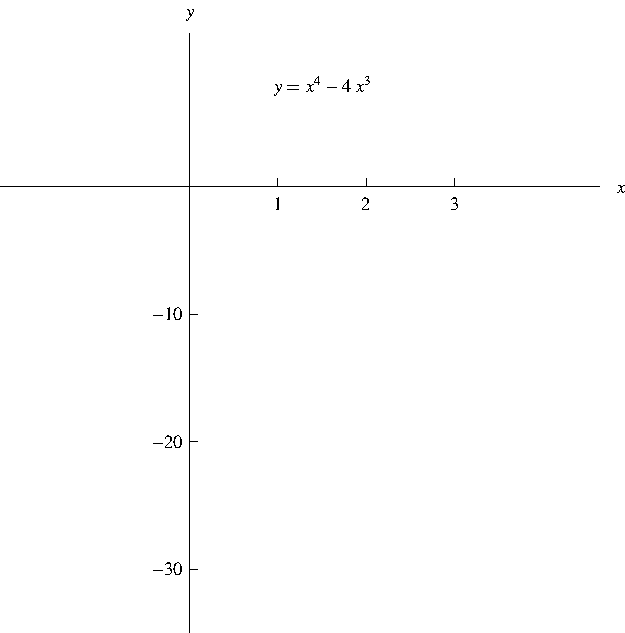
\includegraphics[height=4.5cm]{curve-sketching/pictures/04-03-ex6a.pdf}%
%}%
%\only<handout:0| 20-39>{%
%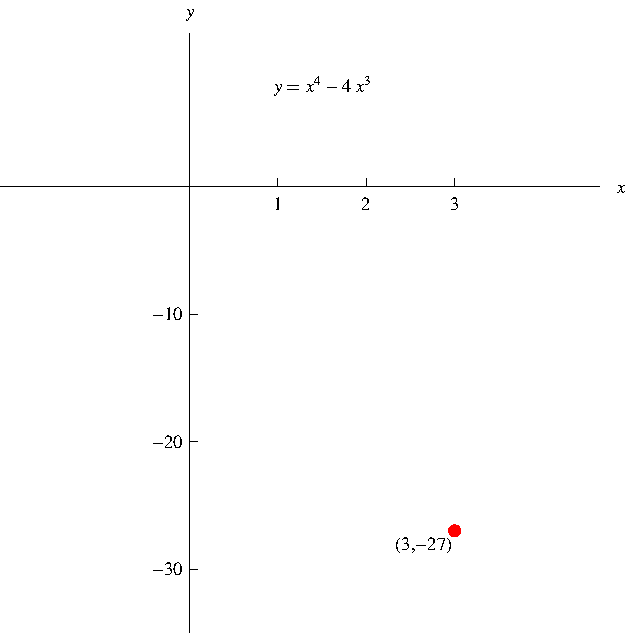
\includegraphics[height=4.5cm]{curve-sketching/pictures/04-03-ex6b.pdf}%
%}%
%\only<handout:0| 40-41>{%
%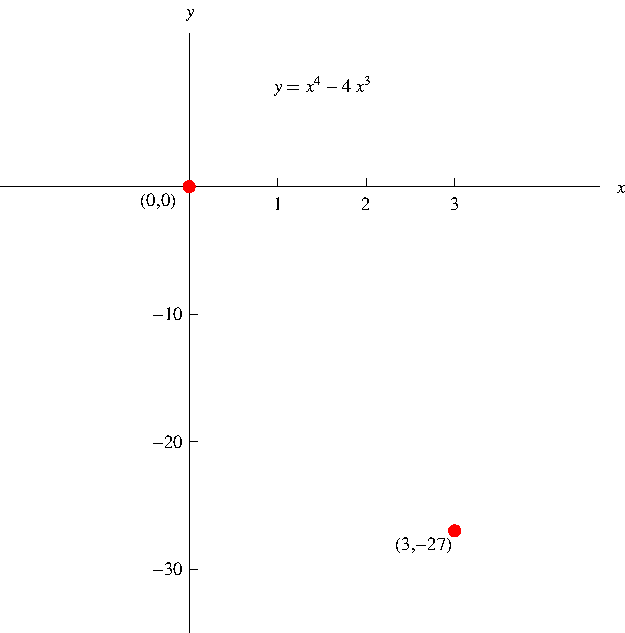
\includegraphics[height=4.5cm]{curve-sketching/pictures/04-03-ex6c.pdf}%
%}%
%\only<handout:0| 42-43>{%
%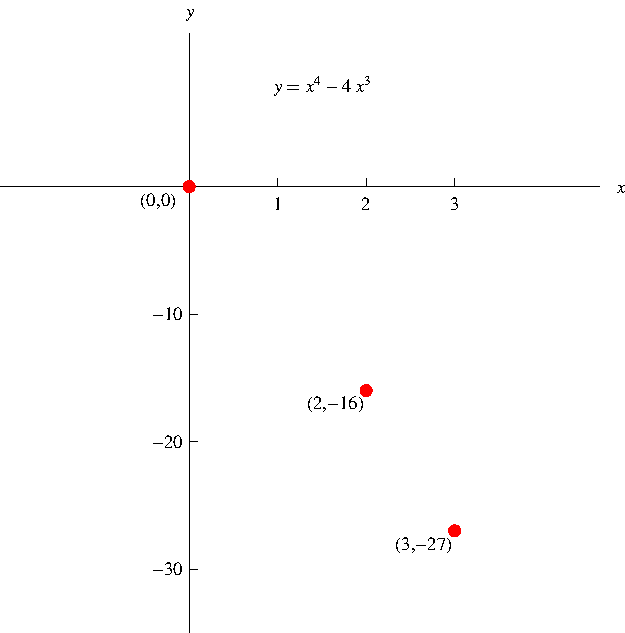
\includegraphics[height=4.5cm]{curve-sketching/pictures/04-03-ex6d.pdf}%
%}%
%\only<handout:0| 44-45>{%
%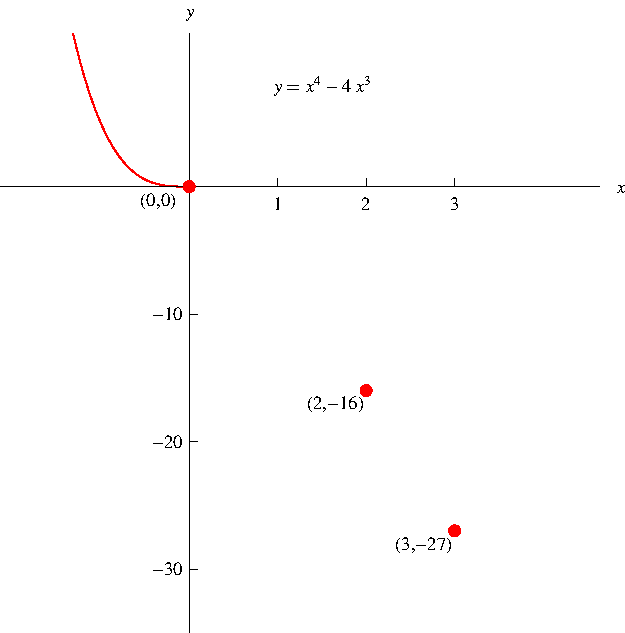
\includegraphics[height=4.5cm]{curve-sketching/pictures/04-03-ex6e.pdf}%
%}%
%\only<handout:0| 46-47>{%
%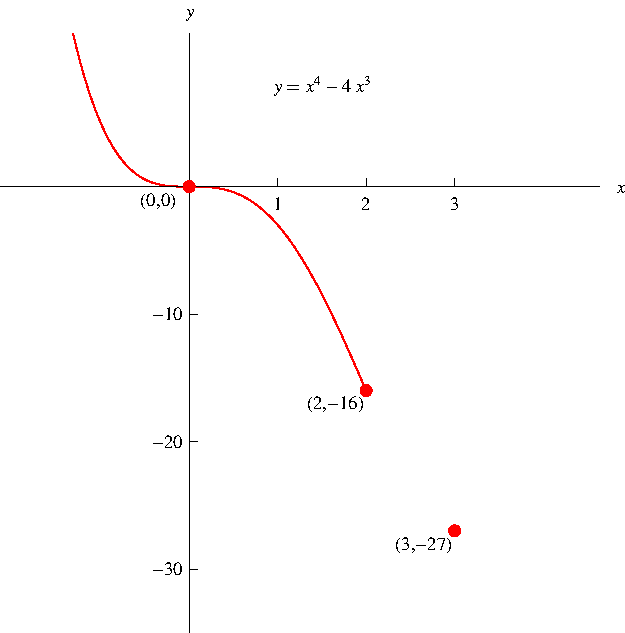
\includegraphics[height=4.5cm]{curve-sketching/pictures/04-03-ex6f.pdf}%
%}%
%\only<48->{%
%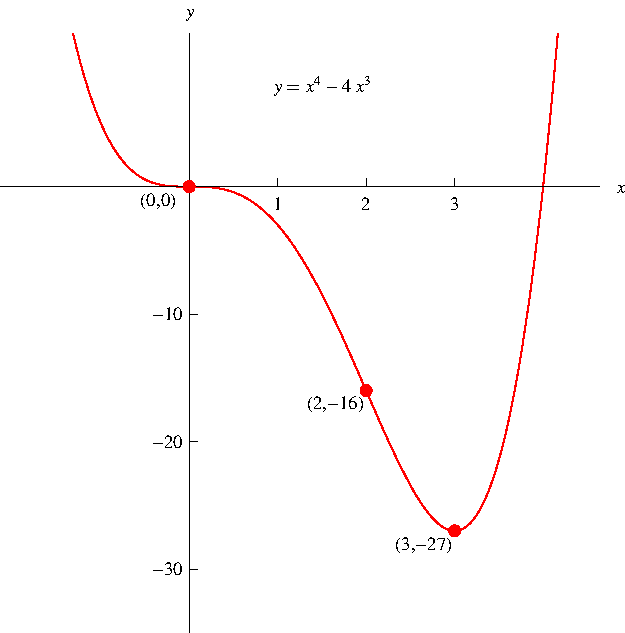
\includegraphics[height=4.5cm]{curve-sketching/pictures/04-03-ex6g.pdf}%
%}%

\vspace{.1in}

\uncover<28->{%
\ \ \ \begin{tabular}{|@{\ }r@{\ }|@{\ }c@{\ }|@{\ }l@{\ }|}
\hline
Interval & $f''(x)$ & \alertNoH{ 35,43-48}{Concave}\\
\hline
\alertNoH{ 29-30,37,43-44}{$(-\infty , 0)$} &%
$\fcAnswer{30}{\alertNoH{ 30,37}{+}}$ &%
\uncover<35->{\alertNoH{ 35,43-44}{up}}\\
\alertNoH{ 31-32,37-38,45-46}{$(0, 2)$} &%
$\fcAnswer{32}{\alertNoH{ 32,37-38}{-}}$ &%
\uncover<35->{\alertNoH{ 35,45-46}{down}}\\
\alertNoH{ 33-34,38,47-48}{$(2, \infty )$} &%
$\fcAnswer{34}{\alertNoH{ 34,38}{+}}$ &%
\uncover<35->{\alertNoH{ 35,47-48}{up}}\\
\hline
\end{tabular}
}%
\column{.60\textwidth}
\begin{itemize}
\item<2-| alert@2-3,23-26>  $f'(x) =  \alertNoH{ 4-5}{\fcAnswer{3}{4x^3 - 12x^2} \uncover<4->{ = }\fcAnswer{5}{4\alertNoH{ 11}{x^2}\alertNoH{ 12}{(x-3)}.}}$
\item<2-| alert@6-7,29-34>  $\alertNoH{ 13-16}{f''(x) = } \alertNoH{ 8-9}{\fcAnswerUncover{2}{7}{\alertNoH{ 13-16}{12x^2 - 24x}} \uncover<8->{ = } \fcAnswer{9}{12x(x-2).}}$
\item<10->  Critical numbers: \fcAnswerUncover{10}{11}{\alertNoH{21-22}{$0$}} and \fcAnswerUncover{10}{12}{\alertNoH{17-18}{$3$}.}
\item<13->  \alertNoH{ 13-14,21-22}{$f''(0) = \fcAnswer{14}{0}$} and \alertNoH{ 15-18}{$f''(3) = \fcAnswer{16}{36 > 0.}$ }
\item<17->  Second Derivative Test:
\item<17-| alert@17-18>  \alertNoH{ 47-48}{Local \fcAnswer{18}{\!\!minimum} at $3$.}  $\alertNoH{ 19-20}{ \uncover<19->{f(3)=\fcAnswer{20}{-27.}}}$
\item<22-| alert@22>  No information about $0$.
\item<23-> First Derivative Test:
\item<23-> \alertNoH{ 23-24}{$f'$ is $\fcAnswer{24}{-}$ on $(-\infty , 0)$} \alertNoH{ 25-26}{and $\fcAnswer{26}{-}$ on $(0, 3)$}.
\item<27-> No local max or min at $0$.
\item<36-> Inflection points: $\alertNoH{ 39-40}{\uncover<39->{(}\fcAnswer{37}{0} \uncover<39->{, \fcAnswer{40}{0})}}$ and $\alertNoH{ 41-42}{ \uncover<39->{(} \fcAnswer{ 38}{2} \uncover<39->{, \fcAnswerUncover{39}{42 }{-16}).}}$
\end{itemize}
\end{columns}
\end{example}
\end{frame}
% end module curve-sketching-ex6
